\documentclass[a4paper]{article}

\usepackage[swedish]{babel}
\usepackage[utf8]{inputenc}
\usepackage{amsmath}
\usepackage{graphicx}
\usepackage{url}

\graphicspath{ {images/} }

\begin{document}

\begin{titlepage}
\centering
{\bfseries\huge Projektplan DAT290}

\vspace{10mm}

{\Large Radiostyrd Bil, Grupp 07}

\vspace{20mm}

{\Large \itshape{Joakim Junttila, Johanna Gudmandsen, Gustav Holst,\\Henrik Klein Moberg, Anders Berggren Sjöblom, \\[1mm] Stanislaw Zwierzchowski, Carl Lundgren}}

\vspace{10mm}

{DATUM}


\normalsize{
\begin{table}[b]
\centering
\begin{tabular}{|l|l|l|}  \hline
          & \bf Namn & \bf Datum   \\ \hline \hline
 Granskad & NAMN     & DATUM        \\ \hline
 Godkänd  & NAMN     & DATUM         \\ \hline
  \end{tabular}  
  \end{table}}

\end{titlepage}
\newpage
\tableofcontents
\newpage


\section{Syfte}
Projektets syfte är att uppgradera en radiostyrd bil till en mer modern teknisk produkt. Genom att ersätta handkontrollen med mer aktuell teknologi blir bilen mer användarvänlig och dess funktioner mer adapterade till dagens standarder.

\section{Mål}
Projektet går ut på att ersätta en del av elektroniken i en radiostyrd bil. Det utgår från en bil där mottagare och sändare i den befintliga styrelektroniken byts ut mot ARM-baserade system. Vidare ska en kontrollapplikation implementeras med hjälp av ett antal avståndsmätare, därefter ska bilen självständigt kunna köra rakt fram i högsta möjliga takt och på ett avstånd av maximalt 1 cm från en vägg bromsa in helt utan att kollidera med väggen. Dessa uppgraderingar ska båda använda sig av Bluetooth. 

Sedan implementeras styrning via en telefonapplikation som ska kunna kontrollera bilen genom ett Androidsystem. Även denna uppgradering ska använda sig av Bluetooth.


\section{Bakgrund}
För att kunna kontrollera en radiobil används en handkontroll(sändare) och en signalomvandlare(mottagare). Radiosignaler på en okänd frekvens skickas från sändaren och avkodas av mottagaren i radiobilen. Dessa omvandlas då till elektroniska signaler som antingen kontrollerar bilens hastighet eller riktning. Parallellt med detta styrs även bilens hastighet av motorns kraftutslag, medan riktningen beror på hjulens gradförskjutning. Genom en ytterligare signal kan bilens hastighet även reverseras. Bilens styrenhet omvandlar radiosignaler som sedan kontrollerar bilens rörelse.

\subsection{Nya styrsignaler}
Bilens styrsignaler kontrolleras av en kontrollenhet, MRX-242. Enheten fungerar simultant som radiomottagare och styrsignalgenerator, och generar signaler till båda motorerna I bilen via tre kablar. I mening att ersätta dessa med nya signaler finns även tillgång till ett ytterligare kopplingsblock. Blocket kopplas mellan MXR-242 och motorerna, och kommer initialt konfigureras att mäta signalerna från den ursprungliga kontrollenheten i bilen. När dessa är kända kommer blocket omkopplas för att generera nya anpassade styrsignaler. 

\section{Systemöversikt}
\subsection{Ersättning sändare}
Den nya konstruktionen omfattas till viss del av en sändare. Denna består av experimentkortet MD407, en bluetoothmodul samt ett gränssnitt som består av potentiometrar och knappar. I ett första steg kommer en radiolänk i 433 MHz-bandet att användas, detta på grund av en enklare implementering.

\subsection{Ersättning mottagare}
Som komplement till sändaren krävs också en ny mottagare. Även mottagaren består av ett MD407-kort och en bluetoothmodul. Detta MD407-kort genererar styrsignaler till befintlig elektronik i bilen som har hand om varvkontroll på elmotorn samt rattutslag.
För att kunna utföra funktionen där bilen ställer sig mot en vägg kommer även mottagaren utrustas med en avståndsmätare. Denna använder sig av ultraljud och mäter tiden det tar för ljud att återvända efter att ha studsat mot väggen.

\subsection{Utökning Androidapplikation}
Utöver grundsystemet så kommer även en applikation till Android att utvecklas. Tanken är att från en mobiltelefon kunna styra bilen på samma sätt som med fjärrkontrollen. Applikationen ska ha ett grafiskt gränssnitt med knappar för att köra bilen framåt, bakåt, svänga vänster samt svänga höger. Till detta tillkommer en knapp som initierar grundsystemets funktion för att ställa sig mot en vägg så under kortast möjliga tid. Det kommer också bli nödvändigt att ha möjligheten att avbryta processen, vilket kommer implementeras i programmet genom att trycka på någon av de övriga knapparna.

\section{Resursplan}

\begin{tabular}{|l|l|l|}  \hline
 \bf Namn                & \bf Mail                                  & \bf Ansvar                 \\ \hline \hline
 Joakim Junttila         & \url{jcb.​junttila@gmail.​com}              & Projektledare              \\ \hline
 Johanna Gudmandsen      & \url{Johanna.gudmandsen@gmail.com}        & Dokumentationsansvarig     \\ \hline
 Gustav Holst            & \url{holst.g@hotmail.se}                  & Systemintegrationsansvarig \\ \hline
 Henrik Klein Moberg     & \url{Ccx555@gmail.com}                    & Loggboksansvarig           \\ \hline
 Anders Berggren Sjöblom & \url{anders_berggren-sjoblom@hotmail.com} & Resursansvarig             \\ \hline
 Stanislaw Zwierzchowski & \url{staszw@openmailbox.org}              & Verifieringsansvarig       \\ \hline
 Carl Lundgren           & \url{carl.lundgren@hotmail.com}           & Granskningsansvarig        \\ \hline
\end{tabular}

\vspace{5mm}
\noindent Under projektet kommer tillgång till små laborationssalar med datorer att ordnas. Salarna för laborationer återfinns i EDIT-huset på Chalmers, vilka har utrustning med mera som kan komma att behövas i projektet. Gruppen kommer ha ett halvt skåp som kan användas till att förvara material. Bokning av andra salar till möten och skrivarbete kommer göras när detta blir nödvändigt, till detta danvänds grupprummen på Chalmers.

Vidare finns även en del hårdvara att tillgå. Från början av projektet ges en radiostyrdd bil ut och handkontrollen till denna. Dessutom kommer en adapter för egen införing av signaler och moduler för bluetooth- och 433MHz-sändning att tillhandahållas. Förutom det behövs också styrutrustning såsom till exempel potentiometer som möjliggör för ett reglerbart motstånd för att styra rattutslag och hastighet. Slutligen finns det även sensorer som mäter avstånd via ultraljud. Begäran av annan hårdvara som kan komma att behövas anges till den teknikansvarige i lärarteamet som då ger ut detta med godkänd anledning.
 
Vad gäller rapportskrivning samt programmerigskod finns det tillgång till ett dokumentationsprogram, Latex, och en versionshanterare, Git. 

\section{Milstolpar}
Milstolpar uppsatta för projektet finns angivna nedan.
\vspace{5mm}

\begin{tabular}{|l|l|l|} \hline
\bf Nr & \bf Beskrivning & \bf Datum \\ \hline \hline
1 & Projektplan inlämnad & 2016-09-11 \\\hline
2 & Kontrollutbyte klar & 2016-09-23 \\ \hline
3 & Undviken kollidering klar & 2016-10-07 \\ \hline
4 & Androidapplikation klar & 2016-10-14 \\ \hline
5 & Demonstrationsförberedelser klara & 2016-10-18 \\ \hline
6 & Projektrapport inlämnad & 2016-10-23 \\ \hline

\end{tabular}

\section{Aktiviteter}
Aktiviteter för projektet finns angiven nedan.
\vspace{5mm}

\begin{tabular}{|l|l|l|} \hline
\bf Nr & \bf Beskrivning                & \bf Tidsåtgång \\ \hline \hline
1      & Sriva dagordningar             & 6   h \\ \hline
2      & Uppdatering loggbok            & 10  h \\ \hline
3      & Projektmöten                   & 65  h \\ \hline
4      & Projektplansskrivning          & 50  h \\ \hline
5      & Oppositionsskrivning           & 9   h \\ \hline
6      & Projektrapportsskrivning       & 250 h \\ \hline
7      & Demonstrationsförberedelser    & 50  h \\ \hline
8      & Granskning och modifiering     & 40  h \\ \hline
9      & Föreläsningar                  & 140 h \\ \hline
10     & Konsultation                   & 10  h \\ \hline 
11     & Förståelse av billaboration    & 60  h \\ \hline
12     & Styrsignalsgenererande         & 100 h \\ \hline
13     & Handkontrollsutbyte            & 100 h \\ \hline
14     & Bluetoothöverskrivning         & 50  h \\ \hline
15     & Undviken väggkollidering       & 200 h \\ \hline
16     & Androidprogrammering           & 60  h \\ \hline 
17     & Dokumentation under laboration & 20  h \\ \hline
\end{tabular}

\section{Tidsplan}

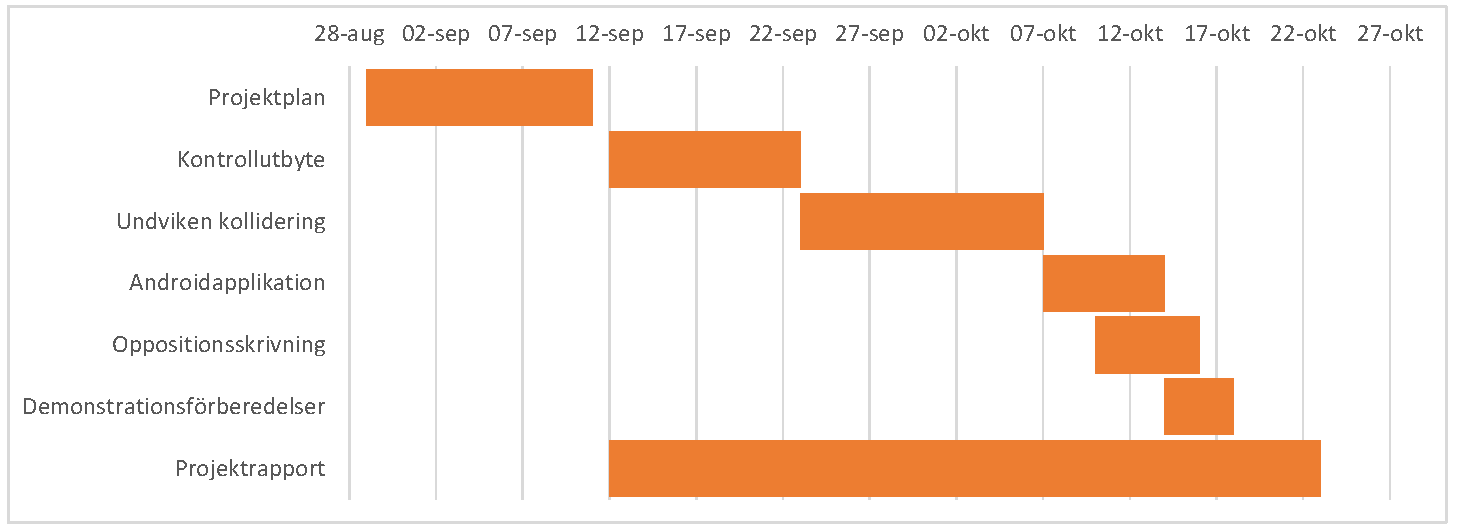
\includegraphics[width=\textwidth]{gantt.pdf}

\section{Mötesplan}

\begin{tabular}{|l|l|l|} \hline
\bf Vad           & \bf Datum  & \bf Var \\ \hline \hline
Projektgruppsmöte & 2016-08-31 &    4207 \\ \hline
Projektgruppsmöte & 2016-09-07 &    4207 \\ \hline
Projektgruppsmöte & 2016-09-14 &    4207 \\ \hline
Projektgruppsmöte & 2016-09-21 &    4207 \\ \hline
Projektgruppsmöte & 2016-09-28 &    4207 \\ \hline
Projektgruppsmöte & 2016-10-05 &    4207 \\ \hline
Projektgruppsmöte & 2016-10-12 &    4207 \\ \hline
Projektgruppsmöte & 2016-10-19 &    4207 \\ \hline
\end{tabular}

\vspace{5mm}
\noindent Behövs det extra mötestid med för kortare, mer specifika möten ordnas grupprum på Chalmers av resursansvarig.



\section{Kommunikationsplan}

\begin{tabular}{|l|l|l|l|} \hline
\bf Vad                  & \bf När    & \bf Till  & \bf Hur               \\ \hline \hline
Mötesprotokoll möte LV1  & 2016-08-31 & Alla      & PP loggbok   (text)  \\ \hline
Dagordning möte LV2      & 2016-09-06 & Alla      & PP loggbok           \\ \hline
Mötesprotokoll möte LV2  & 2016-09-07 & Alla      & PP loggbok   (text)  \\ \hline
Projektplan              & 2016-09-11 & Lärarteam & PP inlämning (LaTeX) \\ \hline
Dagordning möte LV3      & 2016-09-13 & Alla      & PP loggbok           \\ \hline
Mötesprotokoll möte LV3  & 2016-09-14 & Alla      & PP loggbok   (text)  \\ \hline
Dagordning möte LV4      & 2016-09-20 & Alla      & PP loggbok           \\ \hline
Mötesprotokoll möte LV4  & 2016-09-21 & Alla      & PP loggbok   (text)  \\ \hline
Dagordning möte LV5      & 2016-09-27 & Alla      & PP loggbok           \\ \hline
Mötesprotokoll möte LV5  & 2016-09-28 & Alla      & PP loggbok   (text)  \\ \hline
Dagordning möte LV6      & 2016-10-04 & Alla      & PP loggbok           \\ \hline
Mötesprotokoll möte LV6  & 2016-10-05 & Alla      & PP loggbok   (text)  \\ \hline
Utkast projektrapport    & 2016-10-09 & Lärarteam & PP inlämning (LaTeX) \\ \hline
Dagordning möte LV7      & 2016-10-11 & Alla      & PP loggbok           \\ \hline
Mötesprotokoll möte LV7  & 2016-10-12 & Alla      & PP loggbok   (text)  \\ \hline
Oppositionskommentar inl.& 2016-10-16 & Lärarteam & PP inlämning (LaTeX) \\ \hline
Dagordning möte LV8      & 2016-10-19 & Alla      & PP loggbok           \\ \hline
Mötesprotokoll möte LV8  & 2016-10-20 & Alla      & PP loggbok   (text)  \\ \hline
Projektrapport           & 2016-10-23 & Lärarteam & PP inlämning (LaTeX) \\ \hline

\end{tabular}

\vspace{5mm}
\noindent Kommunikation inom gruppen sker främst genom {\it slack}.


\section{Kvalitetsplan}
För att på ett bra sätt isolera eventuella problem samt verifiera funktion och kvalité kommer projektet utföras i flera steg där varje steg är en utökning av det förra som noggrant testas innan det påbörjas. 

\subsection{Styrsignaler}
Först ska samtliga av styrsignalerna som bilens radiomottagare kan skicka till styrkretsen analyseras för att få en förståelse av hur de fungerar och därmed kunna återskapa samma styrsignaler med en egen krets. För att verifiera att analysens resultat är korrekt kommer bilens styrkrets, via kabel, kopplas till en krets som genererar styrsignaler enligt de specifikationerna som analysen har resulterat i. Följande moment ska kunna utföras med samma möjligheter som med bilens inbyggda radiomottagare.
\begin{itemize}  
    \item Svänga höger och vänster med olika rattutslag.
    \item Köra framåt och bakåt med olika hastigheter.
\end{itemize}

\subsection{Enkel trådlös kommunikation}
Dessa styrsignaler ska sedan börja skickas trådlöst. En separat krets ska via kommunikation över 433MHz-bandet kunna bestämma vilka styrsignaler som en inbäddad krets ska skicka till bilens styrmodul. Dessa funktioner kommer verifieras på samma sätt som i det tidigare nämnda testet och ha identiska krav.  

\subsection{Bluetooth}
När det finns trådlös styrningsmöjlighet kommer den tidigare kommunikationsmetoden ersättas med Bluetooth-protokollet som fungerar på ett liknande men utökat sätt. Återigen ska den inbäddade kretsen kunna styra bilen enligt signaler som den separata modulen skickar via Bluetooth. Det ska ske med samma krav som i de förgående testen. Utöver det måste den inbäddade kretsen kunna upprätta en anslutning med den separata modulen vilket kommer kontrolleras i samband med styrningstestet.

\subsection{Avståndsmätare}
Slutligen när avståndsmätaren har implementerats ska denna testas genom körning av bilen mot en vägg och mätning av avståndet till väggen då bilen har stannat. Detta ska utföras ett flertal gånger med olika hastigheter. 

\end{document}